\section{Causal Remedy and Ablations}
\label{sec:remedy-results}

\subsection{Velocity coefficient identifies the active cause}

The velocity-scale intervention in \cref{fig:e16-ablation}a produces a structured dose response. At $\lambda=0$, the velocity field carries the same zero terminal velocity as P-only and retains high ripple. Moving $\lambda$ toward one progressively reduces ripple; the matched value $\lambda=1$ reaches zero median ripple. Overshoot at $1.25$ reintroduces variation, while the wrong sign $\lambda=-1$ is substantially worse. This shape is evidence against an explanation based on merely adding another target component. The component must carry the derivative consistent with the intended motion.\claimtag{C3}

\begin{figure*}[t]
 \centering
 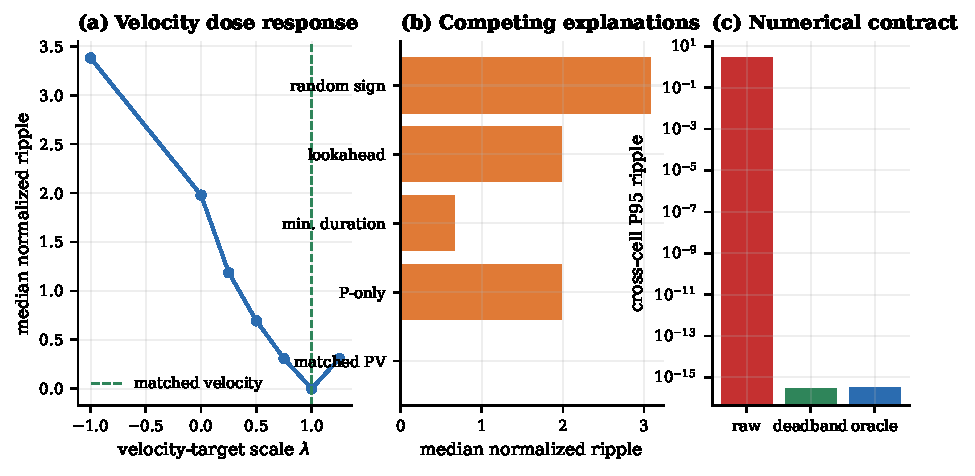
\includegraphics[width=\textwidth]{figures/generated/fig4_e16_ablation.pdf}
 \caption{E16 causal interventions. (a) Velocity-target scale $\lambda$ yields a dose response with an exact minimum at the matched value. (b) Random sign, position lookahead, minimum duration, and P-only retain nonzero median ripple; the bar pools the settings within each tested alternative. (c) Raw \FutureOOne{} leaves a microscopic cross-cell P95 residual, whereas the fixed deadband and oracle PV meet the exact criterion.}
 \label{fig:e16-ablation}
\end{figure*}

Across all \ESixteenArmCount{} arms, matched/oracle PV has median normalized ripple zero and eliminates the rest-to-rest pulse in every tested primary cell. The pooled wrong controls have median ripple \ESixteenWrongRipple. These are exact-profile statements in a single-axis grid; they do not establish that PV is a universal optimum for arbitrary references or objectives. They do establish that matched velocity is the only tested intervention that reproduces the invariant continuation throughout this grid.\claimtag{C3}

\subsection{Lookahead and duration are not exact substitutes}

None of the tested position-lookahead horizons $0,1,2,$ or $5$ reproduces the matched-PV exact profile in every E16 cell. Lookahead changes the requested displacement but leaves the endpoint velocity at zero. It can therefore alter pulse duration or move a configuration across the reachability boundary without repairing the contradiction with constant motion. Likewise, none of the minimum-duration settings off, $T$, $2T$, or $5T$ is an exact equivalent. A duration constraint can delay completion, but it does not require the terminal velocity to equal $\vref$.\claimtag{C4}

These are bounded negative conclusions. A different preview law, a controller that interprets duration differently, or a coupled optimization over several future states could produce another result. E16 shows that the specific tested alternatives do not explain the matched-PV outcome and should not be described as interchangeable repairs. The result is strongest at the level of exact profiles; comparing endpoint positions alone would make several alternatives appear unnecessarily similar.

% Generated; do not edit.
\begin{table*}[t]
\centering
\caption{Causal interpretation of tested target contracts. ``Exact'' refers to the preregistered within-period profile criterion in E16, not only endpoint position.}
\label{tab:causal-ablation}
\small
\begin{tabularx}{\textwidth}{@{}p{0.18\textwidth}p{0.17\textwidth}X X@{}}
\toprule
Intervention & Exact in all tested primary cells? & Observed result & Bounded interpretation \\
\midrule
P-only $(p^\star,0,0)$ & No & repeated rest-to-rest pulses & terminal-state mismatch \\
Matched/oracle PV & Yes & zero median ripple & tested exact remedy \\
Velocity scale $\lambda\ne1$ & No & dose response; wrong sign is worse & derivative value matters \\
Random velocity sign & No & median ripple $3.2007$ & not an extra-DOF effect \\
Position lookahead $0,1,2,5$ & No & no tested horizon reproduces PV & not an exact substitute here \\
Minimum duration off/$1,2,5T$ & No & no tested duration reproduces PV & timing alone is insufficient here \\
Raw Future-O1 & No & microscopic cross-cell residual & implementation-level numerical interaction \\
Future-O1 + $10^{-10}$ deadband & Yes & exact within E16 criterion & tested numerical contract \\
Matched PVA at constant speed & Equivalent to PV & 80 coordinates agree in primary metrics & $a_{\rm ref}=0$ negative control \\
\bottomrule
\end{tabularx}
\end{table*}


\subsection{Causal construction and numerical deadband}

Raw \FutureOOne{} is algebraically exact for the affine schedules in E16, yet floating-point target values create a microscopic residual in some cross-branch cells. The raw method therefore fails the preregistered P95 exactness criterion even though it eliminates macroscopic pulses. Conditioning target velocities within \RecordedDeadband{} of the intended value restores the exact profile in all tested cells. We interpret this as part of the tested numerical contract with Ruckig~\RuckigVersion, not as a universal mathematical requirement for derivative targets.\claimtag{C12}

The recorded fixed-grid targets provide an independent magnitude check on that conditioning scale. Among \RecordedCycleCount{} raw target-velocity entries, exactly \RecordedZeroTargetCount{} are zero, and the smallest nonzero magnitude is \RecordedMinimumNonzeroTarget. It exceeds the E16 deadband by more than an order of magnitude. Applying the same deadband would therefore leave every nonzero recorded target unchanged; no recorded performance gain is being manufactured by truncating small but meaningful velocities. This check establishes target-sequence equivalence, while a later clean replay remains the release-level provenance gate.

\subsection{Matched acceleration as a negative control}

A05 compares matched PV and PVA on constant-speed coordinates. For each finite-difference stencil, the primary stop-and-go metrics agree across \PVAPVEquivalentCoordinateCount{} paired coordinates to the declared tolerance. This is expected from the motion: the matched acceleration is zero, so PVA supplies no additional derivative information. The result is a useful negative control for the mechanism but does not imply that acceleration targets are generally useless. Indeed, nonconstant reference motion and arbitrary target-state OTG are precisely settings in which nonzero target acceleration can matter~\cite{berscheid2021ruckig}.\claimtag{C8}

Together, the interventions support a causal chain: zero terminal velocity produces the pulse when rest-to-rest is reachable; the correct velocity coefficient removes it; wrong values do not; position preview and timing constraints are not exact substitutes in the tested grid; and a history-only construction retains the effect after an implementation-specific numerical conditioning step.
